
%(BEGIN_QUESTION)
% Copyright 2009, Tony R. Kuphaldt, released under the Creative Commons Attribution License (v 1.0)
% This means you may do almost anything with this work of mine, so long as you give me proper credit

Read and outline the introduction and the ``2-Way Solenoid Valves'' subsections of the ``Solenoid valves'' section of the ``Discrete Control Elements'' chapter in your {\it Lessons In Industrial Instrumentation} textbook.  Note the page numbers where important illustrations, photographs, equations, tables, and other relevant details are found.  Prepare to thoughtfully discuss with your instructor and classmates the concepts and examples explored in this reading.

\underbar{file i04193}
%(END_QUESTION)




%(BEGIN_ANSWER)


%(END_ANSWER)





%(BEGIN_NOTES)

2-way valves are like SPST switches: either on or off.

\vskip 10pt

A solenoid valve is a valve operated by an electrical solenoid coil.  The number of ``ways'' is simply the number of fluid ports on the valve.

\vskip 10pt

Solenoid valves are often shown in the same format as fluid power valves: as boxes with flow-direction symbols inside.  The boxes are always drawn in the valve's ``normal'' (resting) position.  When the valve is actuated (energized) the boxes ``slide'' such that different flow-direction symbols line up with the ports to describe what will happen in its active state.  Each actuator symbol {\it pushes} on the boxes rather than {\it pulls} on the boxes, when activated.

$$\includegraphics[width=15.5cm]{i04193x04.eps}$$

$$\includegraphics[width=15.5cm]{i04193x03.eps}$$

Switches and valves, of course, give opposite meanings to the words ``open'' and ``closed'', just to make things confusing.

\vskip 10pt

Arrowheads on flow-direction symbols are often important, because the valve might not be able to stop flow if sufficient pressure is applied the wrong way (against the arrow).  Double-headed arrows are used for valves where there is no preferred direction of flow.  Valves with unidirectional arrows ae designed such that normal operating pressures tend to hold the valve trim in its normal (resting) position.








\filbreak

\vskip 20pt \vbox{\hrule \hbox{\strut \vrule{} {\bf Suggestions for Socratic discussion} \vrule} \hrule}

\begin{itemize}
\item{} Explain how to interpret the ``box'' diagrams used to denote solenoid valves and other fluid-control valves.
\item{} Explain how to identify which ``box'' in a spool-valve symbol is the ``normal'' or ``resting'' state of the valve.
\item{} Define the terms ``open'' and ``closed'' with reference to fluid power valves (rather than electrical switches).
\end{itemize}












\vfil \eject

\noindent
{\bf Prep Quiz:}

Choose the answer that best describes the operation of this fluid control valve:

$$\includegraphics[width=15.5cm]{i04193x01.eps}$$

\begin{itemize}
\item{} It shuts off fluid flow when energized
\vskip 5pt 
\item{} It is actuated by hydraulic pressure
\vskip 5pt 
\item{} It passes fluid flow in all states
\vskip 5pt 
\item{} It passes fluid flow when energized
\vskip 5pt 
\item{} It shuts off fluid flow in all states
\vskip 5pt 
\item{} It is built for handling two-way flow
\end{itemize}


\vfil \eject

\noindent
{\bf Prep Quiz:}

Choose the answer that best describes the operation of this fluid control valve:

$$\includegraphics[width=15.5cm]{i04193x02.eps}$$

\begin{itemize}
\item{} It shuts off fluid flow when energized
\vskip 5pt 
\item{} It is actuated by hydraulic pressure
\vskip 5pt 
\item{} It passes fluid flow in all states
\vskip 5pt 
\item{} It passes fluid flow when energized
\vskip 5pt 
\item{} It shuts off fluid flow in all states
\vskip 5pt 
\item{} It is built for handling two-way flow
\end{itemize}




%INDEX% Reading assignment: Lessons In Industrial Instrumentation, Solenoid Valves (intro)

%(END_NOTES)


